\title{T-61.5130 Machine Learning and Neural Networks}
\author{Karhunen, Luttinen}
\date{Exercise 4, 15.11.2012}

% \usepackage[english]{babel}
% \usepackage[latin1]{inputenc}
% \usepackage{subfigure}
% \usepackage{epsfig}
% \usepackage{amsmath,amssymb}
% \usepackage{psfrag}
% \parindent 0mm
% \textwidth 16cm
% \textheight 23cm
% \oddsidemargin 0cm
% \evensidemargin 0cm
% \topmargin -10mm

\newcommand{\vect}[1]{{\bf{#1}}}
\newcommand{\svect}[1]{\boldsymbol{#1}}
\newcommand{\matr}[1]{\boldsymbol{#1}}


\begin{document}

\maketitle

\begin{enumerate}

\item Construct a MLP network which is able to separate the two
  classes illustrated in Figure \ref{61}. Use two neurons both in the input
  and output layer and an arbitrary number of hidden layer
  neurons. The output of the network should be vector $\left[ 1,
    0\right]^T$ if the input vector belongs to class $\mathcal{C}_1$ and  $\left[ 0,
    1\right]^T$ if it belongs to class $\mathcal{C}_2$. Use nonlinear activation
  functions, namely McCulloch-Pitts model, for all the neurons and
  determine their weights by hand without using any specific learning
  algorithm.
  \begin{itemize}
  \item[(a)] What is the minimum amount of neurons in the hidden layer
    required for a perfect separation of the classes?
  \item[(b)] What is the maximum amount of neurons in the hidden layer?
  \end{itemize}

  \begin{figure}[hbp]
    \centering
    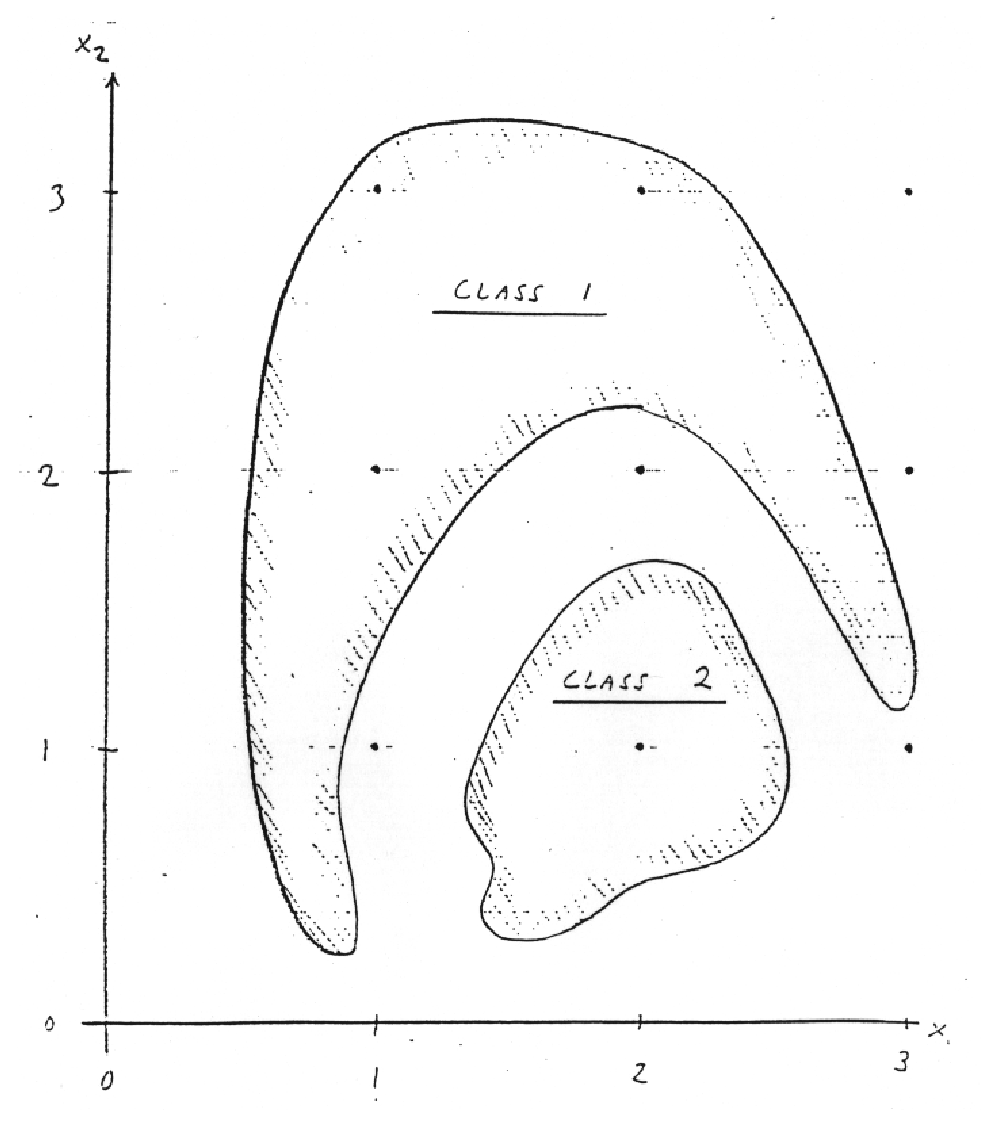
\includegraphics[width=7cm]{mlp_classification.ps}
    \label{61}
    \caption{Classes $\mathcal{C}_1$ and $\mathcal{C}_2$.}
  \end{figure}

  \begin{solution}

    A possible solution:

    \psfrag{x1=1}{$x_1=1$}
    \psfrag{x1=x1}{$x_1=x_2$}
    \psfrag{x2=-x1+4}{$x_2=-x_1+4$}
    \psfrag{w1}{$\vect{w}_1$}
    \psfrag{w2}{$\vect{w}_2$}
    \psfrag{w3}{$\vect{w}_3$}
    \psfrag{w4}{$\vect{w}_4$}
    \psfrag{w5}{$\vect{w}_5$}
    \psfrag{y1}{$y_1$}
    \psfrag{y2}{$y_2$}
    \psfrag{c1}{$\mathcal{C}_1$}
    \psfrag{c2}{$\mathcal{C}_2$}

    \begin{center}
      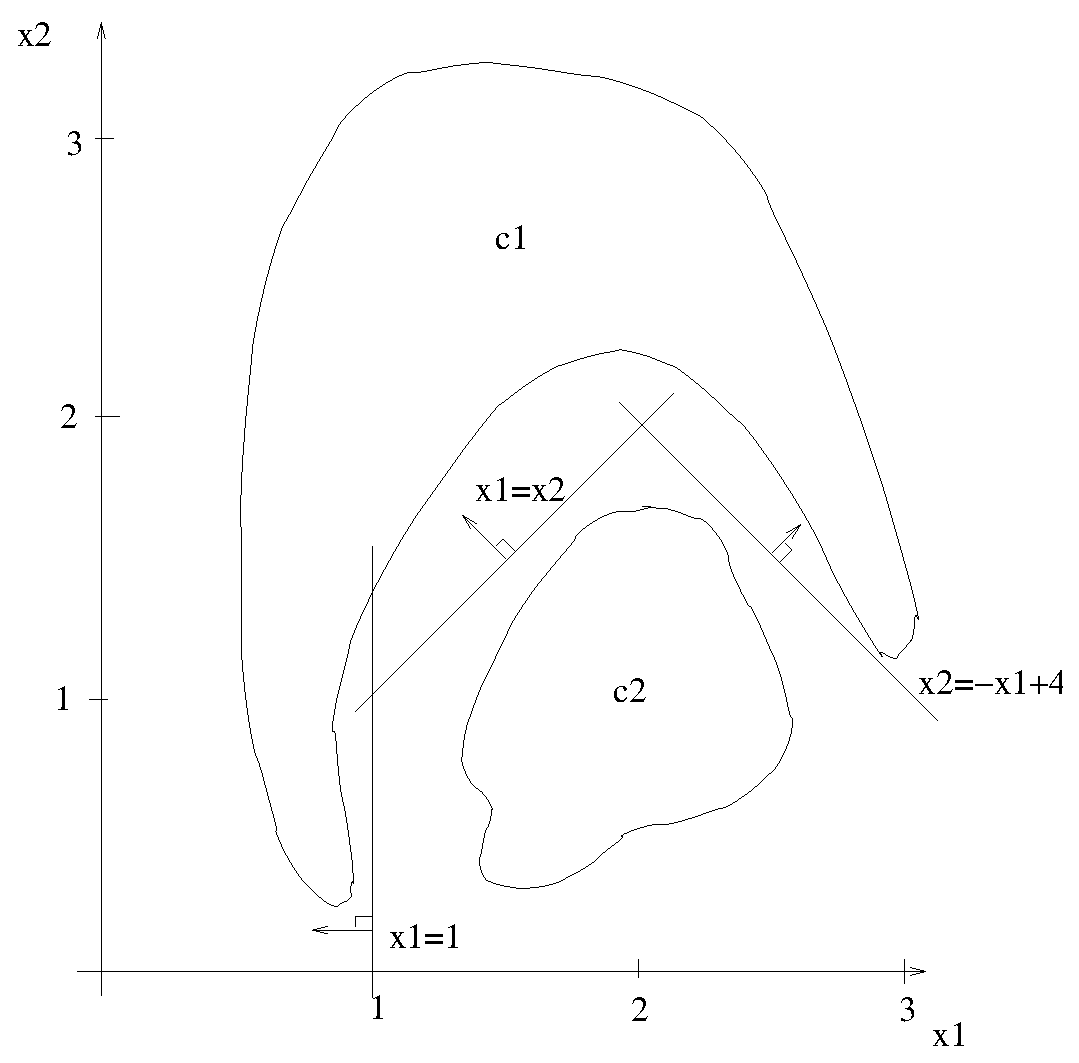
\includegraphics[scale=0.35]{e61.eps}
    \end{center}

    The classification task can be solved using three linear classifiers
    such that $\vect{w}_i^T\vect{x}=0$ gives the classification for each
    linear classifier.

    The network:
    \begin{center}
      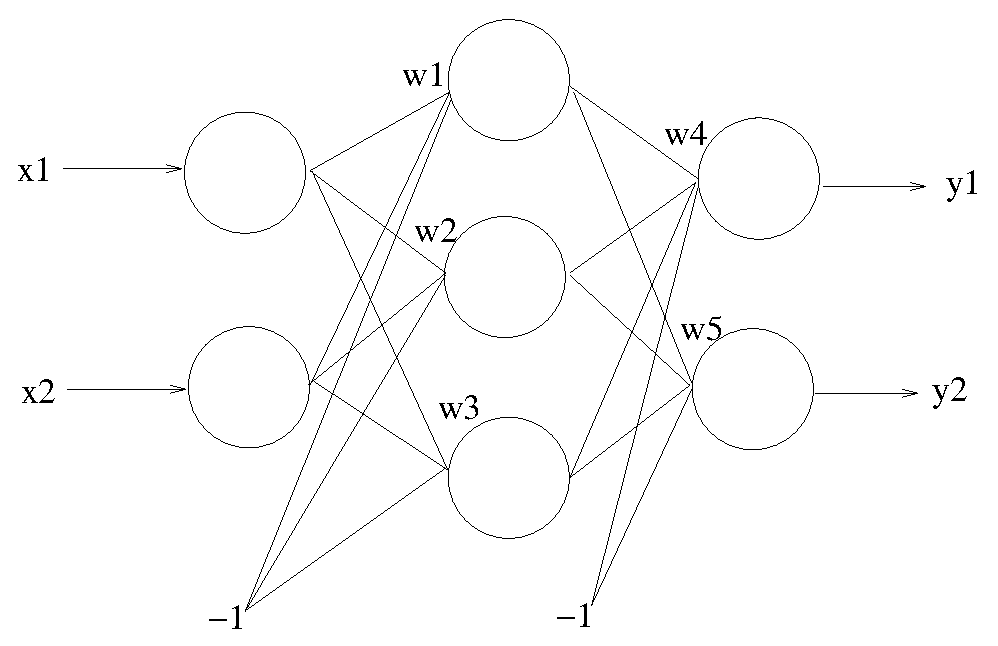
\includegraphics[scale=0.35]{e61-2.eps}
    \end{center}
    % 
    The input relates to the   ${\bf x} = (x_1\ x_2\ \mbox{-1})$.
    From the above figure:
    \begin{equation*}
      \left.
        \begin{array}{l}
          \vect{w}_1=(\begin{array}{ccc}-1&0&-1\end{array})^T\\
          \vect{w}_2=(\begin{array}{ccc}-1&1&0\end{array})^T\\
          \vect{w}_3=(\begin{array}{ccc}1&1&4\end{array})^T
        \end{array}\right\}\mbox{hidden layer}
    \end{equation*}
    The input to the network relates to the coordinate axis by ${\bf x} = (x_1\ x_2\ \mbox{-1})$ the
    last component being the bias.

    Let $z_i \in\{0,1\}$ be the output of the $i$:th hidden layer neuron and $\vect{z}=(\begin{array}{cccc}z_1&z_2&z_3&-1\end{array})^T$.

    The outputs of McCulloch-Pitts perceptrons are determined as follows:
    \begin{equation*}
      z_i=\left\{\begin{array}{l}
          1 \mbox{, if }\vect{w}_i^T\vect{x} > 0\\
          0 \mbox{, otherwise}
        \end{array}\right.
    \end{equation*}

    The weights of the output layer neurons,
    $\vect{w}_4$ and $\vect{w}_5$ are set so that

    $\vect{w}_4=-\vect{w}_5$ and

    $\left\{\begin{array}{l}
        \vect{w}_4^T\vect{z} > 0 \mbox{, if } z_1=1 \mbox{ or } z_2=1 \mbox{
          or } z_3=1\\
        \vect{w}_4^T\vect{z} \leq 0 \mbox{, otherwise}
      \end{array}\right.$

    $\vect{w}_4=\left(\begin{array}{cccc}1&1&1&\frac{1}{2}\end{array}\right)$ is a feasible solution. (The above problem has infinitely many solutions!)
    \begin{enumerate}
    \item[(a)] The minimum amount of neurons in the hidden layer is two as the classes can be separated with two lines.
    \item[(b)] There is no upper limit for the number of hidden layer
      neurons. However, the network might overlearn the training set and
      lose its generalization capability. When the number of hidden layer
      neurons is increased, the boundary between the classes can be
      estimated more precisely.
    \end{enumerate}


  \end{solution}
  
\item The function
  \[
  t(x) = x^2, \hspace{3mm} x \in \left[ 1, 2 \right]
  \]
  is approximated with a neural network. The activation functions of all
  the neurons are linear functions of the input signals and a constant
  bias term. The number of neurons and the network architecture can be
  chosen freely. The approximation performance of the network is
  measured with the following error function:
  \[
  \mathcal{E} = \int_{1}^2 \left[ t({\bf x})-y({\bf x}) \right]^2 d{\bf x}
  \]
  where $\vect{x}$ is the input vector of the network and $y(\vect{x})$ is the
  corresponding response.
  \begin{itemize}
  \item[(a)] Construct a single-layer network which minimizes the error function.
  \item[(b)] Does the approximation performance of the network improve if
    additional hidden layers are included?
  \end{itemize}

  \begin{solution}

    (a) Output of a single-layer network is

    \begin{equation*}
      y(x)=Wx+\theta
    \end{equation*}
    and the approximation performance measure is
    \begin{eqnarray*}
      \mathcal{E}&=&\int_1^2(t(x)-y(x))^2 dx = \int_1^2
      (x^2-Wx-\theta)^2dx\\
      &=&\int_1^2 (x^4+\theta^2 +W^2x^2-2Wx^3+2W\theta x-2\theta x^2)dx\\
      &=&\Big/^2_{\mspace{-11.0mu} 1} \frac{x^5}{5}
      +\theta^2x+\frac{W^2x^3}{3}-\frac{Wx^4}{2}+W\theta x^2-\frac{2}{3}\theta x^3\\
      &=&\frac{31}{5}+\theta^2 +\frac{7}{3}W^2-\frac{15}{2}W+3W\theta-\frac{14}{3}\theta
    \end{eqnarray*}

    Let us find $W$ and $\theta$ which minimize $\mathcal{E}$:
    \begin{equation*}
      \left\{\begin{array}{l}
          \frac{\partial\mathcal{E}}{\partial
            W}=\frac{14}{3}W-\frac{15}{2}+3\theta = 0\\
          \frac{\partial\mathcal{E}}{\partial
            \theta}=2\theta+3W -\frac{14}{3} = 0
        \end{array}\right.
      \Rightarrow
      \left\{\begin{array}{l}
          W^*=3\\
          \theta^*=-2\frac{1}{6}\\
        \end{array}\right.
    \end{equation*}

    As $\left.\begin{pmatrix} \frac{\partial^2\mathcal{E}}{\partial W^2} &
        \frac{\partial^2\mathcal{E}}{\partial W \partial\theta}\\
        \frac{\partial^2\mathcal{E}}{\partial W \partial\theta} &
        \frac{\partial^2\mathcal{E}}{\partial\theta^2}
      \end{pmatrix}\right|_{\begin{array}{l}\scriptstyle  W=W^*\\\theta=\theta^*\end{array}}$
    is positive definite, $\mathcal{E}$ gets its minimum value when
    $W=W^*$ and $\theta=\theta^*$.

    \vspace{0.5cm}
    (b) No because $y(x)=\sum_z w_{1z}^{(n)}\left(\sum_y
      w_{zy}^{(n-1)}\left(\dotsm \sum_a w_{a1}^{(1)}x\right)\dotsm\right) = Wx$. See
    exercise 1, problem 4.

  \end{solution}
  


\end{enumerate}
\end{document}             % End of document.
